\documentclass[10pt,letterpaper]{article}
\usepackage[margin=0.85in]{geometry}
\usepackage{amsmath,booktabs,graphicx,xcolor}
\usepackage[hidelinks]{hyperref}

\setlength{\parindent}{0pt}
\setlength{\parskip}{0.42\baselineskip}
\setlength{\emergencystretch}{1.5em}
\title{\vspace{-1.2em}Adaptive Video Bitrate Selection\\under Varying Network Conditions}
\author{CSE 250A Final Project}
\date{}

\begin{document}
\maketitle
\vspace{-1.5em}

\section{Problem Description}

An adaptive bitrate (ABR) player selects the quality of each video chunk before
downloading it. A higher bitrate improves picture quality, but a slow download
can empty the playback buffer and cause a stall. Large changes between
successive bitrates also carry a cost. We ask whether a tabular Q-learning
policy can use recent download measurements to improve Quality of Experience
(QoE) relative to a fixed-rate policy and a policy that uses buffer occupancy
alone. We also examine which playback costs account for the observed gains
and losses.

\section{Data Sourcing and Processing}

We used 428 FCC and HSDPA bandwidth traces from the public trace
repository~\cite{traces}. Each file contains timestamps and bandwidth in Mbit/s.
We retained zero-bandwidth intervals to represent outages. MERINA provided the
chunk sizes for one video, Mao, with 49 four-second chunks at each of six
bitrates~\cite{merina}.

The imported training partition contained 166 files. The imported holdout set
contained 262 slices from 39 longer recordings. An early split by file placed
slices from 36 recordings in both validation and test. We corrected this by
allocating whole recordings within each source using a deterministic rule
based on a hash of the recording identifier. The resulting manifests contain
166 training, 129 validation, and 133 test files with no recording identifiers
shared across splits. The test files represent only 20 recordings, including
six FCC and 14 HSDPA recordings~\cite{splits}. This matters because adjacent
slices from the same recording can share network conditions.

We also checked training against validation directly. We compared all 166
training files with all 131 original validation files and then with all 129
revised validation files. Both checks returned zero shared filename-derived
recording IDs, zero identical full bandwidth sequences, and zero exact
matches of 16 consecutive samples containing at least two distinct bandwidth
values. Matching the bandwidth column independently of timestamps detects a
copied segment even if its start time changes. These checks can miss copies
that were resampled or otherwise transformed. The 36 confirmed overlaps
were between validation and test. The split and evaluation claims here apply
to the main experiment. In an earlier, separate prototype, 14 of the 20
current test recording IDs appeared in training and two in validation.
The main test thus measures generalization within its own protocol;
some recordings were already known to the broader project~\cite{prototype}.

\section{Modeling and Inference}

\paragraph{Environment and reward.}
We used one trace-driven simulator for all policies. The download delay
depends on the selected chunk size and the bandwidth available over its
transfer, with 95\% payload efficiency and an 80 ms round-trip delay. Playback drains the
buffer during transfer. Time spent with an empty buffer counts as
rebuffering, and a completed download adds four seconds of playback. The
simulator can wrap to the start of a trace when it reaches the end. For
selected bitrate \(b_t\) in Mbit/s and rebuffering duration \(u_t\) in seconds,
the per-chunk reward is
\[
r_t=b_t-4.3u_t-\lvert b_t-b_{t-1}\rvert.
\]
The simulator uses \(b_0=0.75\) Mbit/s for all policies. QoE per video is the sum
of rewards across all 49 chunks~\cite{simulator}.

\paragraph{State, action, and learning.}
Before selecting a bitrate, the agent observes a bin for the harmonic mean of
the most recent three completed-download throughputs, a bin for the current
buffer, and the previous bitrate index. The throughput features use only
completed downloads, with a separate bin before the first download. The
selected discretization has 486 states. The action ladder is 300, 750, 1200,
1850, 2850, or 4300 kbps. We update the table with
\[
 Q(s,a)\gets Q(s,a)+\alpha\left[r+\gamma\max_{a'}Q(s',a')-Q(s,a)\right],
\]
with a target of \(r\) at the final chunk.

Each training episode plays the full video from a random position in a
randomly sampled training trace. Exploration uses an \(\epsilon\)-greedy
policy, with \(\epsilon\) decreasing linearly from 1.0 to 0.01 over the first
80\% of training. A two-round validation search compared discretization,
learning rate, discount, history length, and training schedules. The
selected setting used fine bins, \(\alpha=0.02\), \(\gamma=0.5\), and 30,000
episodes. We retrained that setting with five fresh seeds (100--104) and
evaluated the frozen greedy policies from the beginning of each test trace.

\paragraph{Baselines.}
The fixed policy selects 1200 kbps for every chunk. The buffer-based rule
uses a 10-second reservoir and a 40-second cushion to map buffer occupancy
to a bitrate. The baselines use their declared defaults~\cite{implementation}.

\section{Results and Discussion}

\begin{table}[htbp]
\centering
\small
\caption{Test results across 133 trace files. Q-learning entries show mean
\(\pm\) standard deviation across five training seeds.}
\label{tab:test}
\begin{tabular}{lrrrr}
\toprule
Policy & QoE/video & Bitrate (kbps) & Rebuffer (s/video) & Switches/video \\
\midrule
Fixed 1200 kbps & \(-261.37\) & 1200 & 74.35 & 1.00 \\
Buffer-based & \(36.78\) & 1069 & 1.66 & 14.48 \\
Q-learning & \(39.64\pm1.10\) & \(1176\pm7\) & \(1.97\pm0.11\) & \(12.34\pm1.95\) \\
\bottomrule
\end{tabular}
\end{table}

Q-learning improved average test QoE by 2.86 points over the buffer-based
baseline. Giving each original recording equal weight produced a similar
gain of 2.76 points. The table reports variation across training seeds.
For uncertainty across network conditions, we averaged the five seeds within
each test slice, then resampled whole recordings with replacement, keeping
their slices together. The 95\% percentile interval for the slice-weighted
mean gain was $[0.20, 5.98]$ QoE points (20 recordings, 10,000 draws). The fixed-rate policy incurred over a minute of
stall time per video on average, consistent with its inability to lower the
rate when the connection cannot sustain 1200 kbps~\cite{testresults}.

\subsection{What Accounts for the QoE Gain?}

The reward breakdown explains why a policy with more rebuffering can still
score higher. Across all test traces, the higher bitrates added 5.25 QoE
points per video. Additional stalls cost 1.34 points, and larger cumulative
bitrate changes cost 1.05 points. Q-learning made fewer switches on average,
yet the sum of their magnitudes was higher. The smoothness term penalizes
that sum.

\begin{table}[htbp]
\centering
\small
\caption{Q-learning minus buffer-based QoE per video, decomposed into
signed contributions. The components are rounded independently.}
\label{tab:decomposition}
\begin{tabular}{lrrrr}
\toprule
Test subset & Bitrate & Rebuffering & Switching magnitude & Total \\
\midrule
FCC (45 slices) & \(+5.99\) & \(-0.59\) & \(+0.76\) & \(+6.16\) \\
HSDPA (88 slices) & \(+4.88\) & \(-1.72\) & \(-1.98\) & \(+1.18\) \\
All (133 slices) & \(+5.25\) & \(-1.34\) & \(-1.05\) & \(+2.86\) \\
\bottomrule
\end{tabular}
\end{table}

The gain from selecting higher rates appeared in both networks
(Table~\ref{tab:decomposition}). The difference was how much each policy paid
for that gain. On FCC, the rebuffer cost was small and the switching term
favored Q-learning. On HSDPA, rebuffering and switching costs absorbed most
of the higher-bitrate reward. When whole recordings were resampled within each source, the HSDPA interval
was $[-1.30, 4.26]$ and the FCC interval was $[1.46, 12.02]$. Only six
recordings contributed to the FCC estimate.

\subsection{Two Outcomes Within the Same HSDPA Recording}

Two slices of \texttt{norway\_car\_1} illustrate how the tradeoff changes
within a single recording. We chose the pair with the largest QoE contrast
among same-recording pairs that won in one slice and lost in the other for
all five seeds. The examples illustrate failure and success modes.

\begin{table}[htbp]
\centering
\small
\caption{Buffer-based to Q-learning comparison on two slices of
\texttt{norway\_car\_1}. Q-learning metrics average the five seeds.}
\label{tab:cases}
\begin{tabular}{lrrr}
\toprule
Slice & Bitrate (kbps) & Rebuffering (s) & QoE difference \\
\midrule
\texttt{part0} & \(1712\to2013\) & \(0.56\to0.56\) & \(+21.35\) \\
\texttt{part2} & \(981\to1123\) & \(0.53\to10.87\) & \(-44.02\) \\
\bottomrule
\end{tabular}
\end{table}

On \texttt{part0}, Q-learning selected higher rates without extending the
stall time. On \texttt{part2}, its bitrate reward increased by 7.00 points,
but the extra 10.34 seconds of stalling cost 44.44 points before the
additional switching penalty. To locate the stalls, we replayed the first archived seed (100) and
the buffer rule from the start of \texttt{part2}. Table~\ref{tab:replay}
shows both post-startup stalls for that agent. Its recent throughput estimate
is the harmonic mean of the three completed downloads before the request.

\begin{table}[htbp]
\centering\small
\caption{The two post-startup stalls on \texttt{norway\_car\_1\_part2},
seed 100. Rates are in Mbit/s and times in seconds. Chunks are numbered from 1.}
\label{tab:replay}
\begin{tabular}{rrrrrrr}
\toprule
Chunk & Prior estimate & Chosen rate & Measured rate & Buffer before & Download & Stall \\
\midrule
10 & 1.28 & 1.20 & 0.31 & 8.76 & 14.41 & 5.66 \\
39 & 2.11 & 2.85 & 0.43 & 17.72 & 26.52 & 8.80 \\
\bottomrule
\end{tabular}
\end{table}

At chunk 10 the selected bitrate was below the recent estimate, yet the
realized download throughput fell to 0.31 Mbit/s. At chunk 39 the agent
requested 2.85 Mbit/s with nearly 18 seconds buffered. The request took
26.52 seconds and exhausted that reserve. During this replay, the buffer
rule incurred only the 0.53-second startup wait. Both policies followed the
same recorded link, but their request times depended on earlier decisions.
These two stalls illustrate how much risk a substantial buffer can still
carry when recent downloads overstate throughput for the next request.

\subsection{Does Throughput Predictability Explain the Source Difference?}

FCC samples are spaced five seconds apart, whereas HSDPA samples typically
arrive about once per second. To compare the same time horizon, we formed
duration-weighted five-second windows and used the harmonic mean of the
previous three windows to predict the next one. FCC had lower median
normalized forecast error (0.193 versus 0.219), while HSDPA had higher
lag-one correlation (0.405 versus 0.147). These statistics measure different
properties. Correlation measures persistence, while forecast error measures
the accuracy of a specific predictor.

Across the 133 test slices, three-window forecast error was negatively
correlated with Q-learning's QoE advantage (\(r=-0.464\)). The association
persisted when averaging within each of the 20 original recordings
(\(r=-0.628\)). Mean bandwidth and variability were also associated with the
gain. In addition, fixed-time link bandwidth differs from the actual chunk
throughput measured by the agent. The results are consistent with a benefit
from more informative throughput observations. Establishing the mechanism
would require controlling for bandwidth and examining the policy's decisions
around stalls~\cite{dynamics}.

\clearpage
\begin{figure}[htbp]
\centering
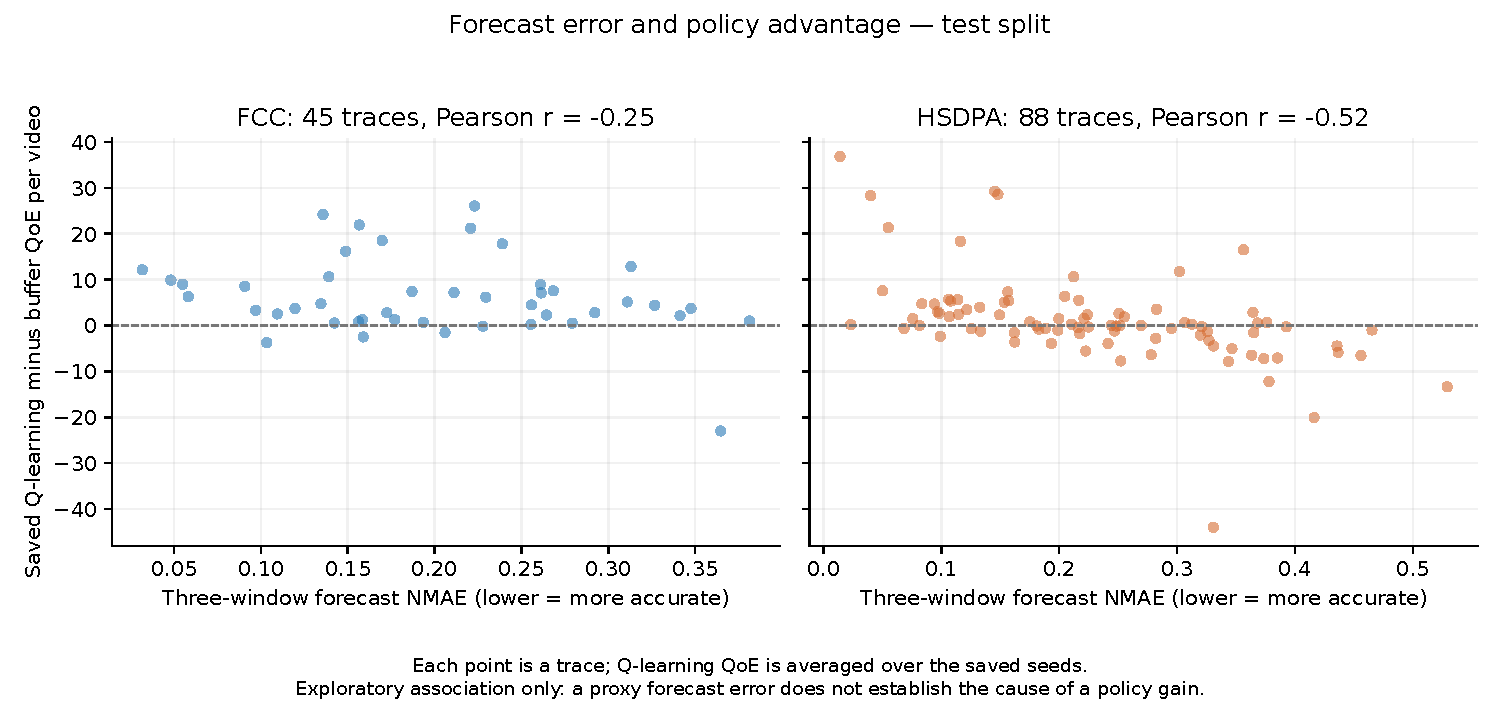
\includegraphics[width=0.83\linewidth]{images/test_qoe_relationship.pdf}
\caption{The gain over buffer-based adaptation is often larger at lower
normalized forecast error. Each point represents a test slice. Slices can
share an original recording.}
\label{fig:forecast}
\end{figure}

\subsection{Validation Stability and Scaling}

Fine discretization appeared throughout the top validation configurations,
and lower learning rates and shorter discount horizons performed better in
the explored grid. Several leading configurations were within roughly one
seed standard deviation, so the exact ranking is uncertain. About 35\% of
the fine-bin states were unvisited during training. Increasing the number of
bins would create more entries to estimate, especially for rare combinations
of throughput and buffer. The current experiments support a useful policy
under the selected settings. They leave open how the policy would behave
with other videos or under a tuned buffer baseline~\cite{implementation}.

\paragraph{Shorter training budget.}
We trained the selected configuration for 10,000 episodes with the original
five tuning seeds (0--4) and evaluated the greedy policies on the same 129
validation traces. The exploration rate decayed over the first 80\% of each
run, and the remaining hyperparameters were held fixed. Validation QoE was
\(44.43\pm1.33\), compared with \(46.48\pm1.97\) for the archived 30,000-episode
setting (\href{https://github.com/Bobby-Zhu/abr-q-learning/blob/2169df2/results/q_learning/tuning.csv}{round-two tuning results}).
These values are the mean and sample standard deviation across seeds.
Using one third of the training episodes cost 2.05 QoE points on average.
The comparison supports keeping the 30,000-episode budget for the reported
configuration.

\section{Conclusion}

On the shared simulator, tabular Q-learning achieved higher average QoE than
the two baseline policies. The gain came mainly from selecting higher
bitrates and was clearest on FCC. The HSDPA examples show how quickly stalls
can outweigh an apparent gain in picture quality. The evaluation used one
video, a small number of source recordings, and untuned baseline defaults.
The replay suggests a specific follow-up on validation. Compare the frozen
policy with a variant that discounts recent throughput when downloads have
varied sharply. Track bitrate gains and stall costs separately, including
when the buffer exceeds ten seconds. A validation-tuned buffer rule and
additional videos would test how far these findings generalize.

\clearpage
\appendix
\section{State Bins and Reproduction}

The selected throughput bin edges in Mbit/s are 0.4, 0.7, 1.0, 1.4, 1.9,
2.6, and 3.5. The buffer edges in seconds are 2, 4, 7, 10, 14, 19, 26, and
35. Observations on an edge are assigned to the upper bin. The team
repository records the manifests, selected configuration, test outputs, and
analysis scripts used by the report at commit \texttt{007a5c1}. The companion
scripts \texttt{replay\_case.py}, \texttt{check\_splits.py}, and
\texttt{recording\_intervals.py} reproduce the chunk replay, overlap checks,
and recording-level resampling from the saved inputs.

\begin{thebibliography}{9}
\bibitem{traces}
Nuowen Kan. \emph{Real-world bandwidth traces}. MIT-licensed data repository.
\href{https://github.com/confiwent/Real-world-bandwidth-traces/tree/d28c4fd48d0e358db024cc0217b111c070815fa7}{Source and version}.

\bibitem{merina}
Nuowen Kan. \emph{MERINA}. MIT-licensed simulation code and chunk metadata.
\href{https://github.com/confiwent/merina/tree/dfd01b7f664e3a9fa0d123945081f7af2ebb31f7}{Source and version}.

\bibitem{splits}
Project team. \emph{Deterministic trace splits}.
\href{https://github.com/Bobby-Zhu/abr-q-learning/blob/2169df2/data/splits/README.md}{Split documentation} and
\href{https://github.com/Bobby-Zhu/abr-q-learning/pull/1}{recording-level split fix}.

\bibitem{simulator}
Project team. \emph{ABR simulator and reward configuration}.
\href{https://github.com/Bobby-Zhu/abr-q-learning/blob/2169df2/docs/SIMULATOR.md}{Repository documentation}.

\bibitem{implementation}
Project team. \emph{Tabular Q-learning for ABR}.
\href{https://github.com/Bobby-Zhu/abr-q-learning/blob/2169df2/docs/Q_LEARNING.md}{Training and evaluation protocol} and
\href{https://github.com/Bobby-Zhu/abr-q-learning/pull/2}{implementation PR}.

\bibitem{testresults}
Project team. \emph{Frozen test comparison}.
\href{https://github.com/Bobby-Zhu/abr-q-learning/blob/2169df2/results/final/test/summary.md}{Summary},
\href{https://github.com/Bobby-Zhu/abr-q-learning/blob/2169df2/results/final/test/per_trace.csv}{per-slice metrics}, and
\href{https://github.com/Bobby-Zhu/abr-q-learning/blob/2169df2/results/trace_dynamics/per_recording.csv}{recording-level summaries}.

\bibitem{dynamics}
Project team. \emph{Trace dynamics analysis}.
\href{https://github.com/Bobby-Zhu/abr-q-learning/blob/2169df2/docs/TRACE_DYNAMICS.md}{Methods, figures, and interpretation}.
\bibitem{prototype}
Project team. \emph{Earlier exploratory prototype}.
\href{https://github.com/Bobby-Zhu/abr-q-learning/blob/1c8251acc07a97f89b18e78ff958b8d3b061339e/prototype/results/run_01/manifest.csv}{Run manifest}.
\end{thebibliography}
\end{document}
